\subsection{Extended Kalman Filter (EKF)}\label{subsec:EKF}
The EKF combines the Dead Reckoning prediction step implementation with an implementation of the measurement update step from Equation \ref{eq:bayes_measurement_update}.
This study's EKF uses a 2D Iterative Closest Point (ICP) scan matching algorithm to produce 

The EKF fuses the Dead Reckoning prediction with the ICP measurement update. 
Because the system is non-linear, the EKF linearizes the measurement models using Jacobians \cite{thrun2005probabilistic}.
An illustration of the EKF node is shown in Figure \ref{fig:ekf}.
A KD-Tree is utilized to encode the OccupancyGrid to efficiently find the nearest neighbor in the reference map for each projected LiDAR point.

Because the odometry runs at a higher frequency than the LiDAR does, Odometry messages are buffered in the Odometry callback.
In the LiDAR callback, the odom buffer is emptied and the predict step is performed on each reading.
Next ICP is performed to determine the observed state $z_t$ and match error $\mathcal{M}$.
These values are then fed into the measurement update step shown below.

\begin{figure}[!htbp]
    \centering
    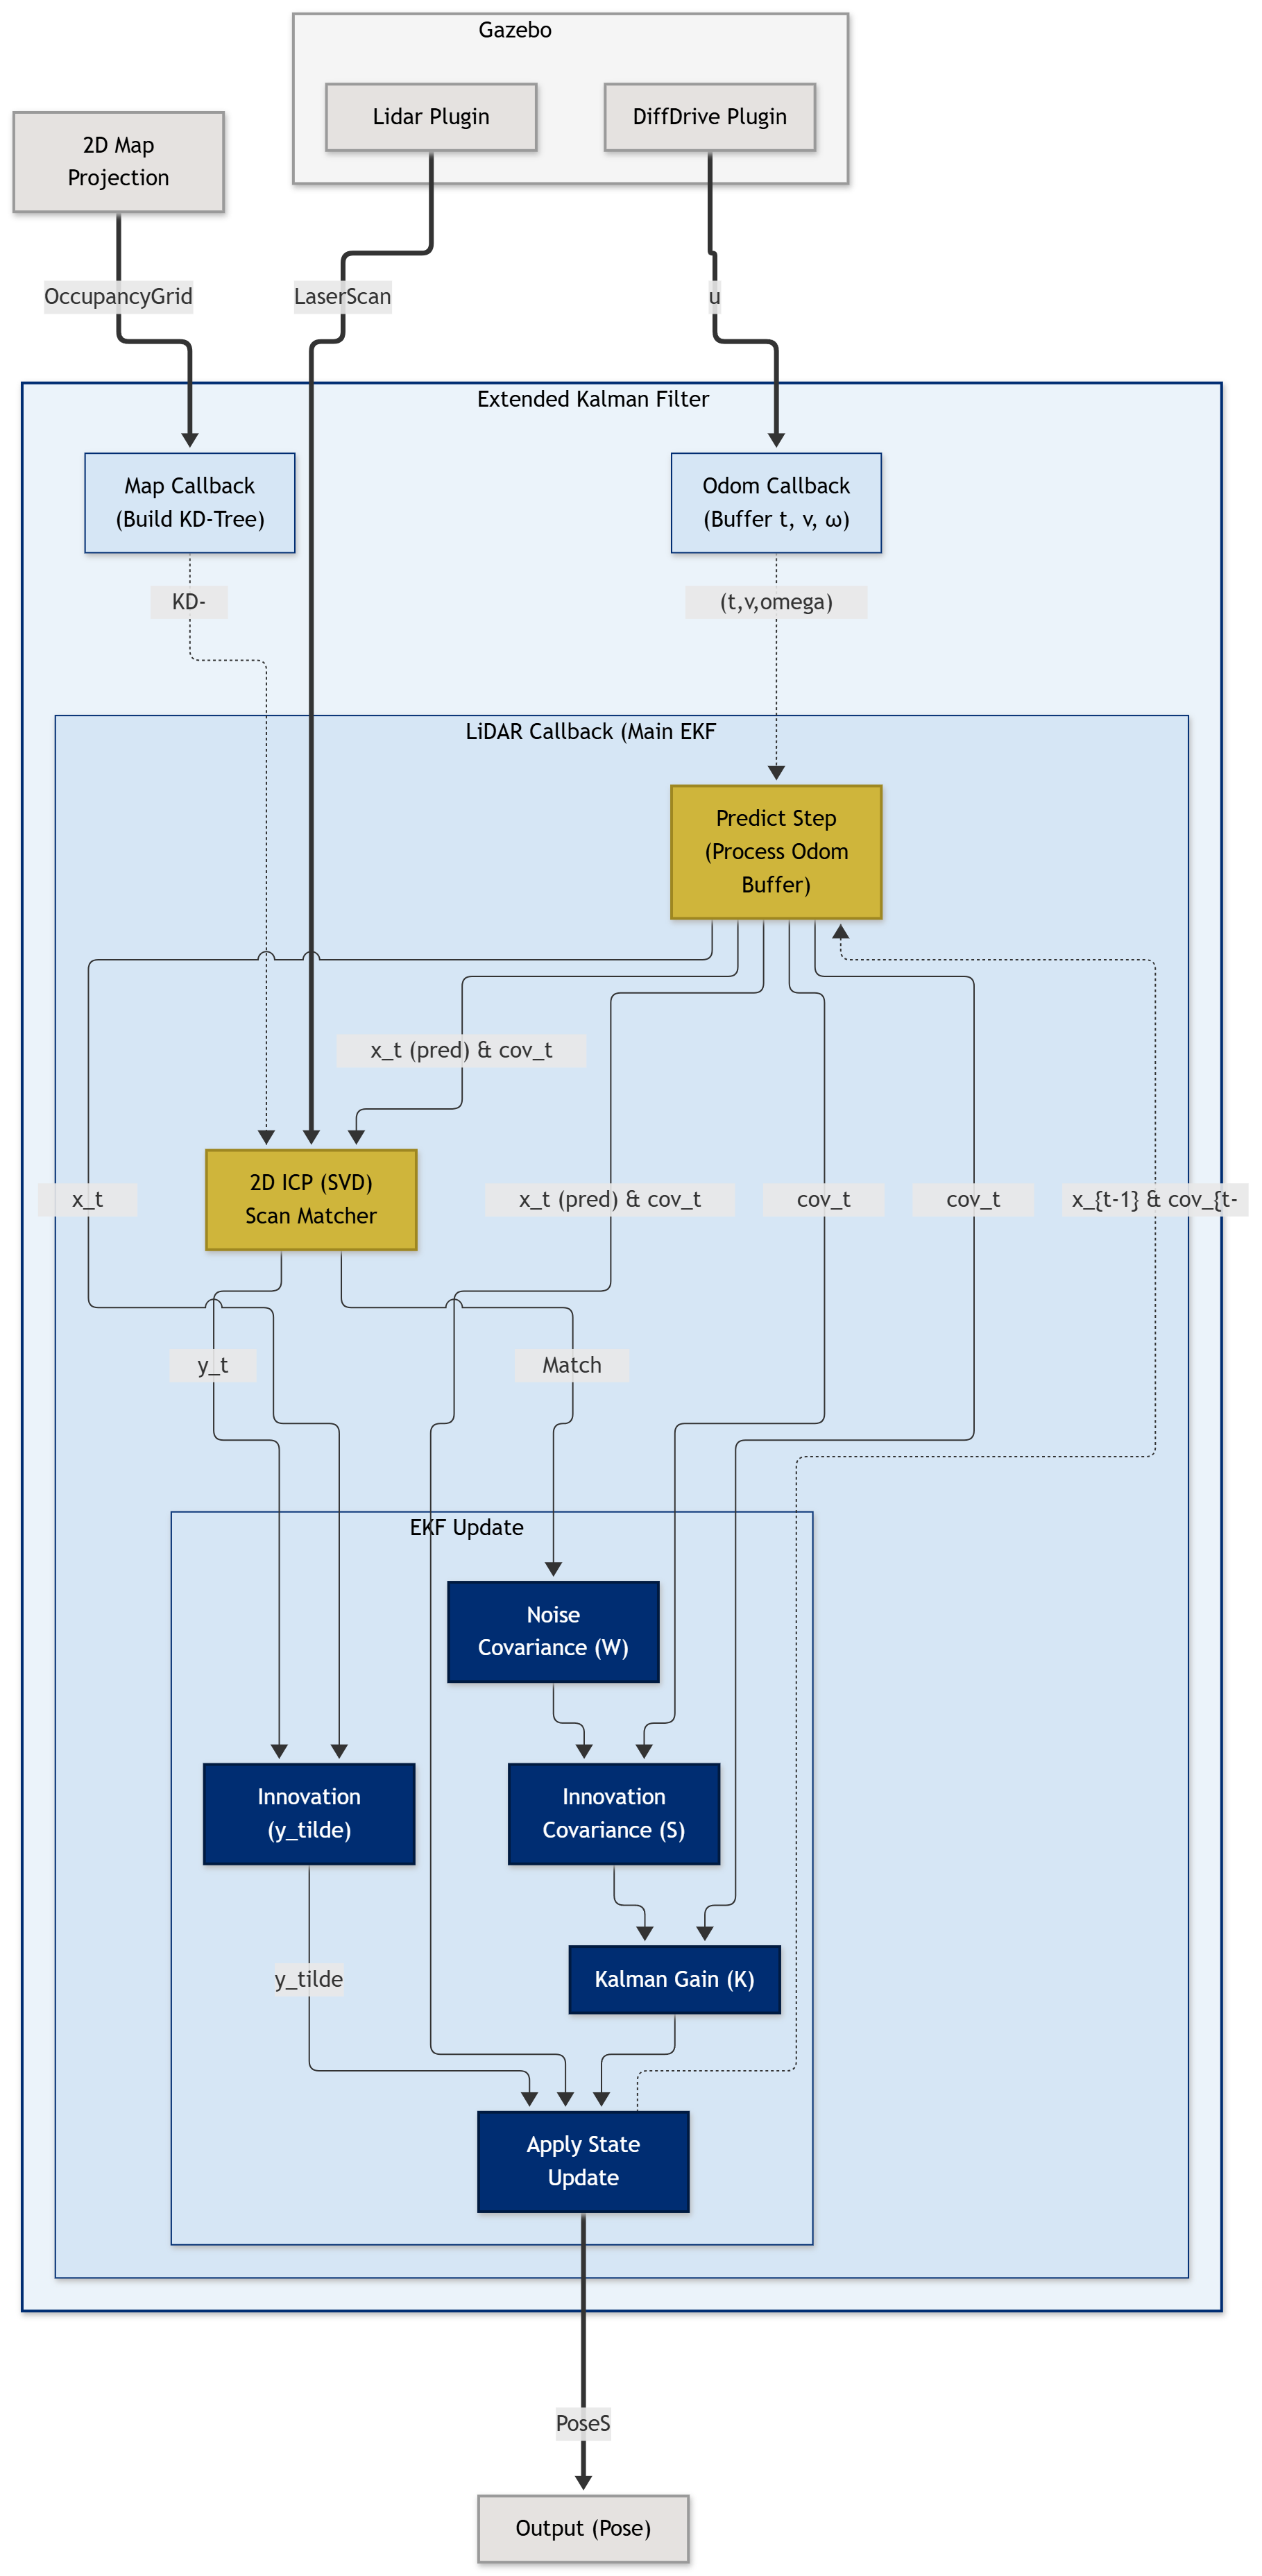
\includegraphics[width=0.65\textwidth]{figures/ekf.png}
    \caption{Extended Kalman Filter Update Algorithm}
    \label{fig:ekf}
\end{figure}

\subsubsection{Augmented Motion Model}\label{subsec:augmented-model}
During initial testing, there was a yaw-rate error that would build up in the EKF.
To mitigate this error, an augmented motion model was designed to include the state and the initial belief for the yaw-rate error which is shown in Equation \ref{eq:Augmented-State}.

\begin{equation}\label{eq:Augmented-State}
    \xi = \begin{bmatrix}
        x \\ y \\ \theta \\ s
    \end{bmatrix}
\end{equation}

The related covariance matrix is defined as $\textbf{P}\in\mathbb{R}^{4\times4}$ and the state and covariance are initialized as $\textbf{x}_0=[0,0,0,1]^T$ and $\textbf{P}_0=\text{diag}(0.1^2, 0.1^2, (5\pi/180)^2, 0.3^2)$.
Therefore the filter begins by assuming the odometry is unbiased ($\widehat{s}=1$), with a standard deviation of 0.3.

\textbf{Forward Kinematics} Substituting true yaw rate $s\omega$ for $\omega$ in Equation \ref{eq:discrete_unicycle_kinematics} and apending $s$.

\begin{equation}\label{eq:kinematics_augmented}
    f_a(\textbf{x},\textbf{u},\Delta t) = \bar{\textbf{x}}_t = \begin{bmatrix}
        x + v \cos(\theta) \Delta t \\ y + v \sin(\theta) \Delta t \\ \theta + s\omega \Delta t \\ s
    \end{bmatrix}
\end{equation}

\textbf{State Jacobian:} The state Jacobian $\textbf{A}_t$ is calculated by finding the partial derivatives of equation \ref{eq:discrete_unicycle_kinematics} with respect to $\textbf{x}$.

\begin{equation}\label{eq:state_jacobian_augmented}
    \textbf{A}_t = \frac{\partial \textbf{f}_a}{\partial \xi} = 
    \begin{bmatrix} 
        1 & 0 & -v \sin(\theta) \Delta t & 0 \\
        0 & 1 &  v \cos(\theta) \Delta t & 0 \\
        0 & 0 & 1                        & \omega \Delta t \\
        0 & 0 & 0                        & 1
    \end{bmatrix}
\end{equation}

\textbf{Control Jacobian:} The control Jacobian $\textbf{G}_t$ is calculated by finding the partial derivatives of equation \ref{eq:discrete_unicycle_kinematics} with respect to $\textbf{u}$.

\begin{equation}\label{eq:control_jacobian_augmented}
    \textbf{G}_t = \frac{\partial \textbf{f}_a}{\partial \textbf{u}} = 
    \begin{bmatrix} 
        \cos(\theta) \Delta t & 0  \\
        \sin(\theta) \Delta t & 0  \\
        0 & \Delta t \\
        0 & 0
    \end{bmatrix}
\end{equation}

\textbf{Process noise:} The process noise equation \ref{eq:mapped_process_noise} is then modified below to include a scaling factor for yaw $q_s$:

\begin{equation} \label{eq:mapped_process_noise_augmented}
    R_t = G_t M_t G_t^T \Delta t + \text{diag}(0,0,0,q_s^2 \Delta t)
\end{equation}

\subsubsection{Prediction}

The EKF prediction step is nearly identical to the Dead Reckoning process described in Section \ref{subsec:Dead-Reckoning:Prediction} except the Augmented Motion Model described in Section \ref{subsec:augmented-model} was used instead of the unicycle motion model.

\subsubsection{Measurement Update}
The observed pose $\textbf{z}_t$ and match error $\mathcal{M}$ come from Iterative Closest Point.
The observation matrix is the identify $H$.

\begin{equation}
    \textbf{H} = \begin{bmatrix}
        1 & 0 & 0 & 0 \\
        0 & 1 & 0 & 0 \\
        0 & 0 & 1 & 0
    \end{bmatrix}
\end{equation}

The innovation is found by Equation \ref{eq:ekf-innovation-cov}.

\begin{equation}\label{eq:ekf-innovation-cov}
    \tilde{y}_t = \textbf{z}_t - \hat{x}_t
\end{equation}

And the innovation covariance is found by Equation \ref{eq:ekf-innovation-cov}.

\begin{equation}\label{eq:ekf-innovation-cov}
    S_t = H \hat{\Sigma}_t H^T + W_t
\end{equation}

A $\chi^2$ statistical acceptance test is then performed to determine statistical acceptance using $\alpha=0.95$ and df$=3$.
If the observation is stastically reasonable, the Kalman gain $\textbf{K}$ is found by Equation \ref{eq:ekf-kalman-gain}

\begin{equation}\label{eq:ekf-kalman-gain}
    K = \hat{\Sigma} H^T S^{-1}
\end{equation}

Finally the state and covariances are updated as follows:
\begin{equation}\label{eq:ekf-state-update}
    \textbf{x}_t = \hat{x} + K \tilde{y}
\end{equation}

\begin{equation}\label{eq:ekf-cov-update}
    \Sigma_t = (I - K H) \hat{\Sigma}
\end{equation}

\textbf{Scan Matching via ICP and SVD:} 
The ICP algorithm implemented follows point-to-point descriptions from \textit{A Review of Point Cloud Registration Algorithms for Mobile Robotics} \cite{pomerleau2015review}.
It uses the predicted values $\bar{\textbf{x}_t}$ and $\bar{\Sigma_t}$, as well as, a KD-Tree built from the OccupancyGrid to output an observed state $\textbf{z}_t$ and a match error $\mathcal{M}$.
The \texttt{LaserScan} is processed into $\mathcal{P}$ and $\mathcal{Q}$ which represent the laser points in the localframe and the nearby collision points in the local frame, respectively.
First the centroid of the point clouds are found by:
\begin{equation}
    \mu_p = \frac{1}{K} \sum_{k = 1}^{K} p_k
\end{equation}

\begin{equation}
    \mu_q = \frac{1}{K} \sum_{k = 1}^{K} q_k
\end{equation}

The covariance is found as follows:

\begin{equation}
    \textbf{H} = \sum_{k = 1}^{K} (p_k - \mu_p) (q_k - \mu_q)^T
\end{equation}

Single Value Decomposition (SVD) is then used to find optimal transformation.
Let $\textbf{U}\varLambda \textbf{V}^T$ be the single value decomponsition $H$.
Then the optimal transformation to minimize the least squared error is shown in Equations \ref{eq:optimal-rotation} and \ref{eq:optimal-translation}:

\begin{equation}\label{eq:optimal-rotation}
    \widehat{R} = \textbf{V}\textbf{U}^T
\end{equation}

\begin{equation}\label{eq:optimal-translation}
    \widehat{t} = \mu_q - \widehat{R}\mu_p
\end{equation}

The observed pose $\textbf{z}_t$ is then found by applying the optimal transformation to $\bar{x}_t$.
The implementation of the EKF node and algorithm can be found in Appendix \ref{subsec:EKF implementation}.
